\documentclass[tikz,border=0pt]{standalone}
\usepackage{tikz}
\usetikzlibrary{calc, shapes, backgrounds}

% --- 颜色定义 ---
\definecolor{AntYellow}{HTML}{FFCC00} % 背景黄
\definecolor{NetGray}{HTML}{808080}    % 网络连线灰
\definecolor{NodeFill}{HTML}{999999}   % 节点填充灰

% --- 使用 tikzset 定义 ant pic ---
\tikzset{
    ant/.pic={
        \begin{scope}[line cap=round]
            % 1. 腿 (Legs)
            \foreach \side in {-1, 1} {
                \draw[black, thick] (0.05*\side, 0.1) -- (0.25*\side, 0.25) -- (0.35*\side, 0.5);
                \draw[black, thick] (0.05*\side, 0) -- (0.3*\side, 0) -- (0.4*\side, -0.1);
                \draw[black, thick] (0.05*\side, -0.15) -- (0.25*\side, -0.3) -- (0.35*\side, -0.5);
            }
            % 2. 触角 (Antennae)
            \draw[black, semithick] (0.05, 0.35) -- (0.15, 0.5) -- (0.1, 0.6);
            \draw[black, semithick] (-0.05, 0.35) -- (-0.15, 0.5) -- (-0.1, 0.6);
            
            % 3. 身体 (Body)
            \fill[black] (0, -0.35) ellipse (0.14 and 0.22);
            \fill[black] (0, 0) ellipse (0.08 and 0.12);
            \fill[black] (0, 0.28) ellipse (0.1 and 0.1);
            
            % 4. 颚 (Mandibles)
            \draw[black, thick] (0.04, 0.36) -- (0.06, 0.42);
            \draw[black, thick] (-0.04, 0.36) -- (-0.06, 0.42);
        \end{scope}
    }
}

\begin{document}

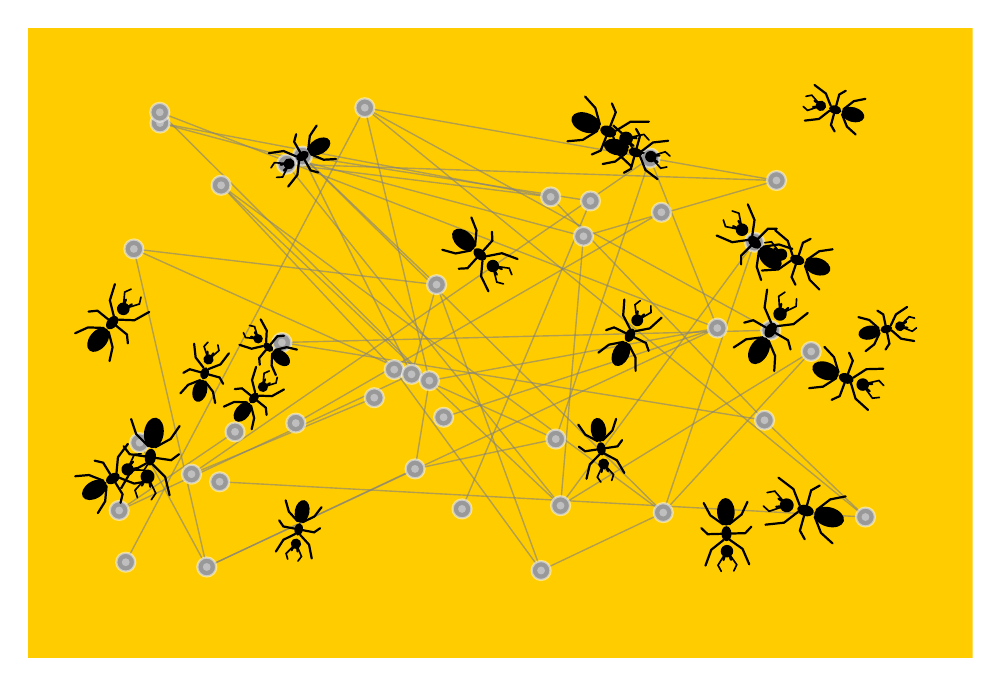
\begin{tikzpicture}
    % =========================================
    % 1. 绘制背景
    % =========================================
    \clip (0,0) rectangle (12, 8);
    \fill[AntYellow] (0,0) rectangle (12, 8);

    % =========================================
    % 2. 绘制群体场 (网络层)
    % =========================================
    \pgfmathsetseed{42}
    
    % 生成 40 个节点
    \foreach \i in {1,...,40} {
        \pgfmathsetmacro{\x}{1 + 10*rnd}
        \pgfmathsetmacro{\y}{1 + 6*rnd}
        \coordinate (N-\i) at (\x, \y);
    }

    % 绘制连线 (使用更稳健的判断逻辑)
    \begin{scope}[opacity=0.6, line width=0.5pt, NetGray]
        \foreach \i in {1,...,40} {
            \foreach \j in {1,2,3} {
                % 计算目标节点索引
                \pgfmathtruncatemacro{\target}{mod(\i+\j, 40)+1}
                
                % --- 修复核心 ---
                % 生成一个0或1的随机整数
                \pgfmathtruncatemacro{\shouldDraw}{rnd < 0.4 ? 1 : 0}
                
                % 如果结果为1,则画线
                \ifnum\shouldDraw=1
                    \draw (N-\i) -- (N-\target);
                \fi
                % --- 修复结束 ---
            }
        }
    \end{scope}

    % 绘制节点
    \foreach \i in {1,...,40} {
        \fill[NodeFill] (N-\i) circle (0.12);
        \draw[white, thick, opacity=0.5] (N-\i) circle (0.12);
        \fill[NetGray!50] (N-\i) circle (0.05);
    }

    % =========================================
    % 3. 绘制蚂蚁 (智能体层)
    % =========================================
    \foreach \k in {1,...,18} {
        \pgfmathsetmacro{\ax}{1 + 10*rnd}
        \pgfmathsetmacro{\ay}{1 + 6*rnd}
        \pgfmathsetmacro{\rot}{360*rnd}
        \pgfmathsetmacro{\scl}{0.6 + 0.3*rnd}
        \path (\ax, \ay) pic[rotate=\rot, scale=\scl] {ant};
    }

    % 特殊位置的蚂蚁
    \path (N-5) pic[rotate=45, scale=0.8] {ant};
    \path (N-12) pic[rotate=120, scale=0.7] {ant};
    \path (N-30) pic[rotate=-30, scale=0.85] {ant};

\end{tikzpicture}

\end{document}